%!TEX program = xelatex
% Note: this template must be compiled with XeLaTeX rather than PDFLaTeX
% due to the custom fonts used. The line above should ensure this happens
% automatically, but if it doesn't, your LaTeX editor should have a simple toggle
% to switch to using XeLaTeX.

\documentclass[
  aspectratio=169, % Uncomment to use an aspect ratio of 16:9 (160 mm by 90 mm)
  %aspectratio=43, % Uncomment to use an aspect ratio of 4:3 (128mm by 96mm)
  t, % Top align all slide content by default
  onlytextwidth, % Typeset content in columns at text width
  10pt, % Default font size, use 10pt for the 16:9 aspect ratio and 8pt for the 4:3 aspect ratio
]{beamer}

\usepackage{../../ImperialTheme/beamer/beamerthemeImperial} % Use the Imperial theme
\usepackage{tikz}
\usetikzlibrary{calc}

\def\imagefolder{../../ImperialTheme/beamer/Images}
\def\Rey{\text{Re}}
\title{jeff update} % Presentation title to appear on the title slide and left footers

\subtitle{} % Presentation subtitle to appear on the title slide

\author{Víctor Ballester} % Author name(s) to appear on the title slide

\date{\today} % Presentation date to appear on the title slide and right footers

\begin{document}

\begingroup
\setbeamercolor{background canvas}{bg=ICLLightGrey} % Slide background color
\setbeamercolor{title page title}{fg=ICLBlue} % Title text color
\setbeamercolor{title page subtitle}{fg=ICLBlue} % Subtitle text color
\setbeamercolor{author}{fg=ICLBlue} % Author(s) text color
\setbeamercolor{date}{fg=ICLBlue} % Date text color
\setbeamertemplate{title page}[logo]{\imagefolder/ICL_Logo_Blue.pdf} % Imperial logo color, use 'ICL_Logo_White.pdf' for white and 'ICL_Logo_Blue.pdf' for blue
\frame[plain, s]{\titlepage} % Output the title page with no footer ('plain') and vertically distributed text ('s')
\endgroup

\begin{frame}
	\frametitle{Linear instability results}
\begin{columns}[T] % [T] ensures correct vertical alignment
		\begin{column}{0.31\linewidth} % Left column
			\begin{itemize}
			  \item We know now that the first linear instability to appear in 2d is a Hopf.
			  \item The $\delta^*$ depends on Ma. Should we leave it as is or fix it to a standard value (e.g. incompressible value, for example)?
			\end{itemize}
		\end{column}
		\begin{column}{0.68\linewidth} % Left column
		      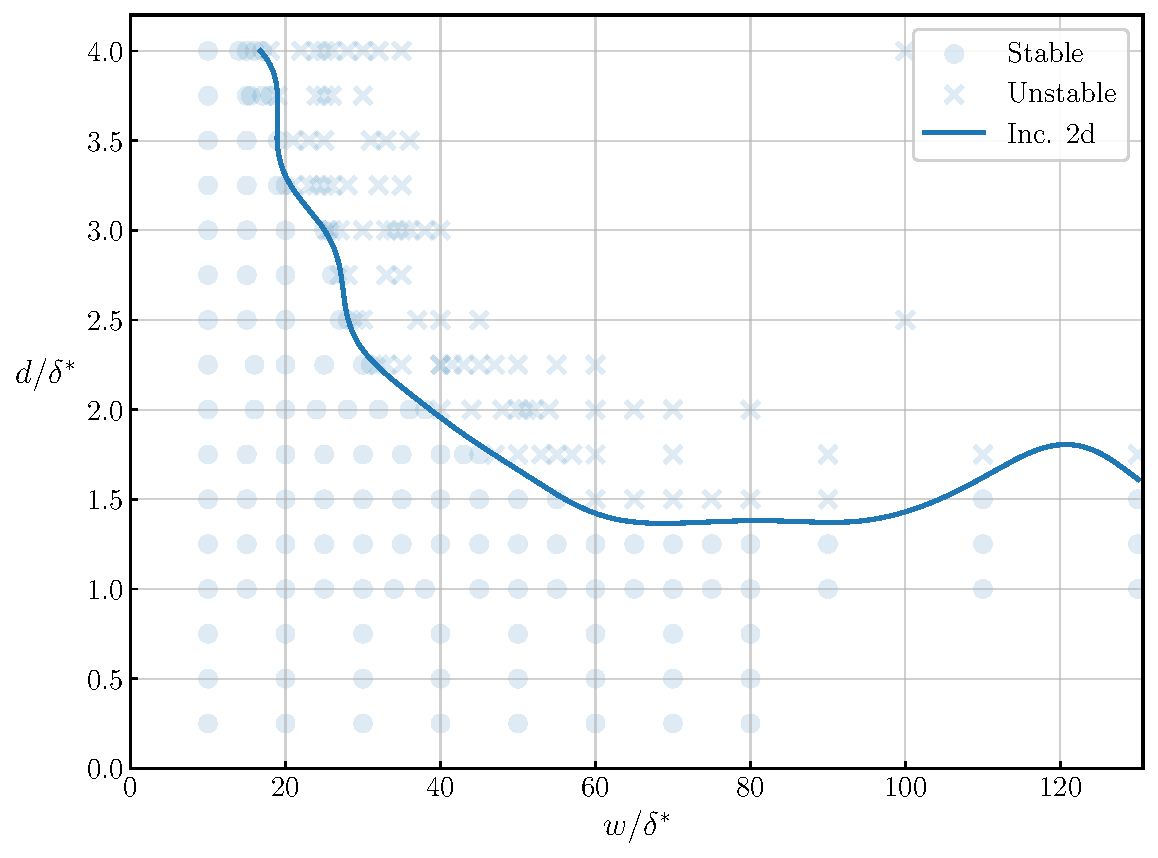
\includegraphics[width=\linewidth]{../../../images/stabilityCurve.pdf}
		\end{column}
	\end{columns}
\end{frame}
\begin{frame}
	\frametitle{Linear instability results}
\begin{columns}[T] % [T] ensures correct vertical alignment
		\begin{column}{0.31\linewidth} % Left column
		About limit $d/w\approx$ large
		  \begin{itemize}
		    \item In general we observe a shift in the onset of instability to lower values of $w$ (at fixed $d$) when increasing Ma until eventually (I think) reaching a limit (which could be imposed by domain restrictions).
			\item A 3d instability located in the gap appears before the Ma = 0.8 2d instability.
		  \end{itemize}
		\end{column}
		\begin{column}{0.68\linewidth} % Left column
	\begin{tikzpicture}
		\node[inner sep=0] (img) {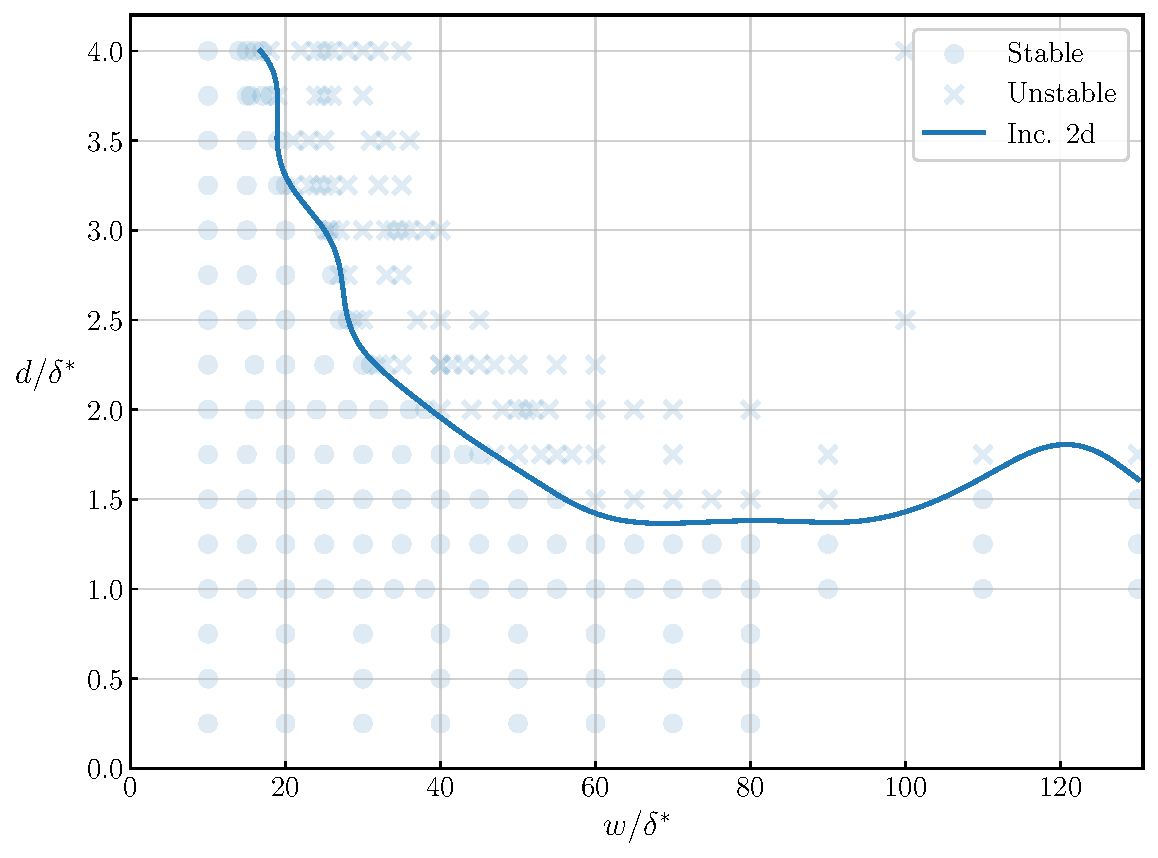
\includegraphics[width=\linewidth]{../../../images/stabilityCurve.pdf}}; % replace with your file
		% Draw a rectangle border (no fill) around some region of the image.
		% Coordinates relative to the image node anchors:
		% (img.north west), (img.south east), etc. We shift the corners to get the square we want.
		\draw[line width=1.5pt, red]
		($(img.north west)+(0.07\textwidth,-0.007\textwidth)$) rectangle
		($(img.north west)+(0.30\textwidth,-0.3\textwidth)$);

	\end{tikzpicture}
		\end{column}
	\end{columns}
\end{frame}
  \begin{frame}
	\frametitle{Linear instability results}
\begin{columns}[T] % [T] ensures correct vertical alignment
		\begin{column}{0.31\linewidth} % Left column
		About limit $d/w\approx$ small
		  \begin{itemize}
		    \item My feeling is that in the limit, 2d instabilities appear before 3d ones (even in the inc case). In the picture it cannot be properly appreciated because I didn't have enough baseflows to run the 3d stability analysis at higher $w$ values, but all the $d = 1.5$ run in 3d became stable.
		    \item Interestingly, Ma = 0.8 bifurcates after Ma = 0.6 at some particular depths.
		  \end{itemize}
		\end{column}
		\begin{column}{0.68\linewidth} % Left column
	\begin{tikzpicture}
		\node[inner sep=0] (img) {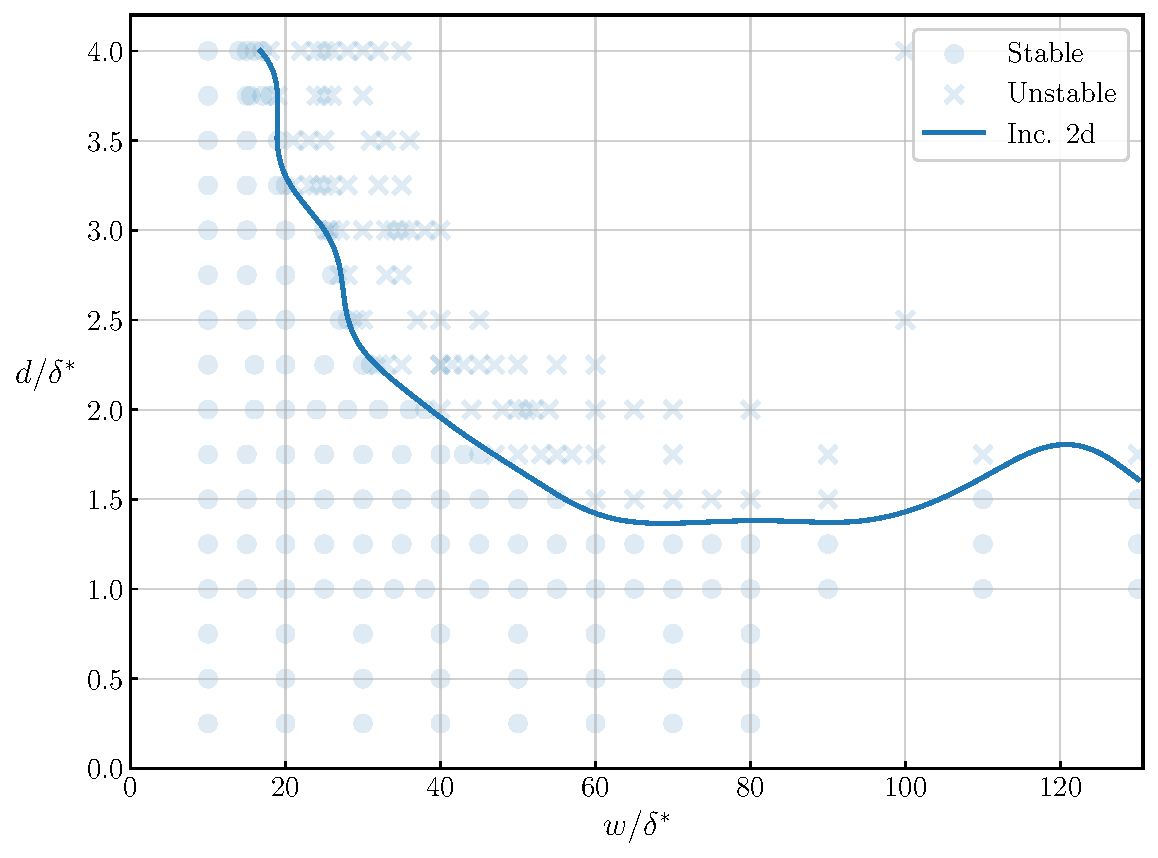
\includegraphics[width=\linewidth]{../../../images/stabilityCurve.pdf}}; % replace with your file
		% Draw a rectangle border (no fill) around some region of the image.
		% Coordinates relative to the image node anchors:
		% (img.north west), (img.south east), etc. We shift the corners to get the square we want.
		\draw[line width=1.5pt, green!70!black]
		($(img.south west)+(0.07\textwidth,0.3\textwidth)$) rectangle
		($(img.south west)+(0.60\textwidth,0.001\textwidth)$);

	\end{tikzpicture}
		\end{column}
	\end{columns}
\end{frame}
  \begin{frame}
	\frametitle{Linear instability results}
\begin{columns}[T] % [T] ensures correct vertical alignment
		\begin{column}{0.31\linewidth} % Left column
		About limit $d/w\approx$ small
		  \begin{itemize}
			  \item Also instabilities seems to appear at lower $d$ in the compressible case compared to the incompressible runs. For example, there is an unstable configuration at $d=1.25$ and $w \gtrsim 35$ for Ma = 0.6, while in the incompressible case all the runs at $d=1.25$ were stable (in the range $w\in [10,100]$).
		  \end{itemize}
		\end{column}
		\begin{column}{0.68\linewidth} % Left column
	\begin{tikzpicture}
		\node[inner sep=0] (img) {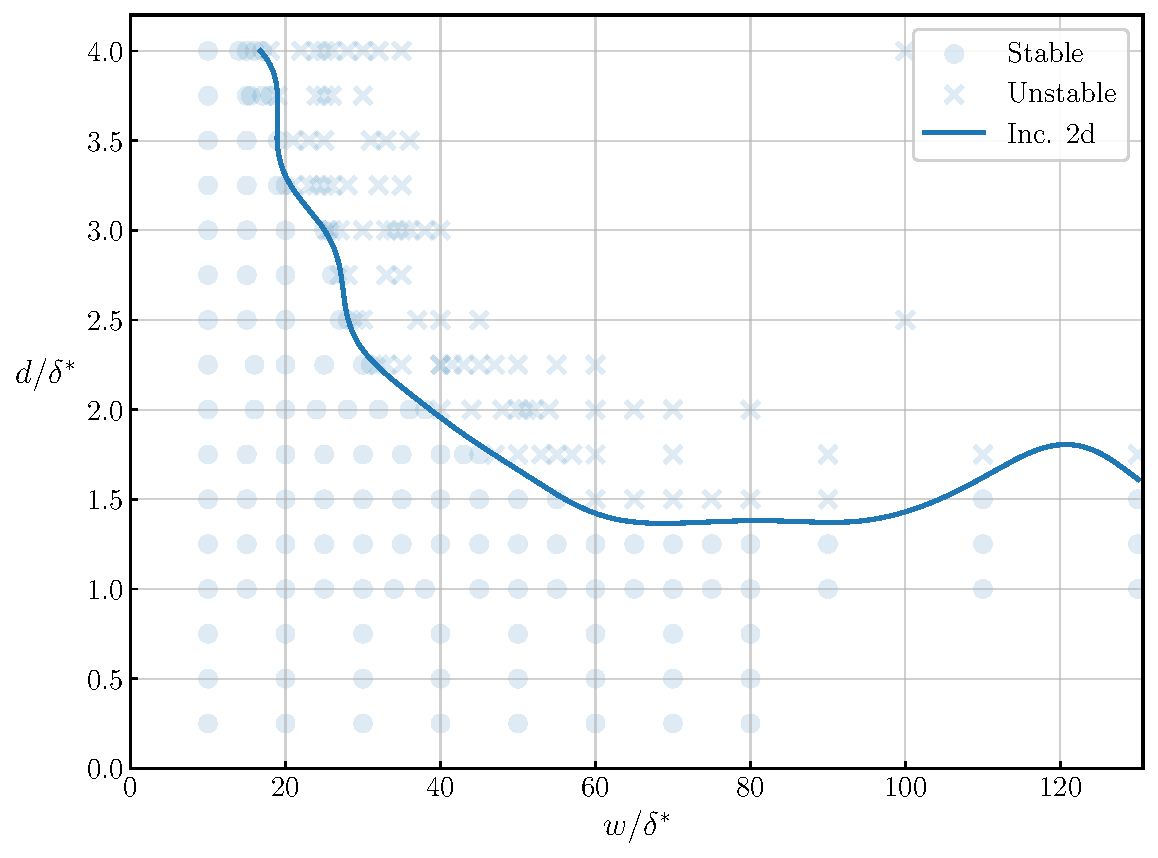
\includegraphics[width=\linewidth]{../../../images/stabilityCurve.pdf}}; % replace with your file
		% Draw a rectangle border (no fill) around some region of the image.
		% Coordinates relative to the image node anchors:
		% (img.north west), (img.south east), etc. We shift the corners to get the square we want.
		\draw[line width=1.5pt, green!70!black]
		($(img.south west)+(0.07\textwidth,0.3\textwidth)$) rectangle
		($(img.south west)+(0.60\textwidth,0.001\textwidth)$);

	\end{tikzpicture}
		\end{column}
	\end{columns}
\end{frame}
\begin{frame}
	\frametitle{Unstable mode comparison d = 2.5}
\begin{columns}[T] % [T] ensures correct vertical alignment
		\begin{column}{0.49\linewidth} % Left column
		  $w = 20$, Ma = 0.6:
		  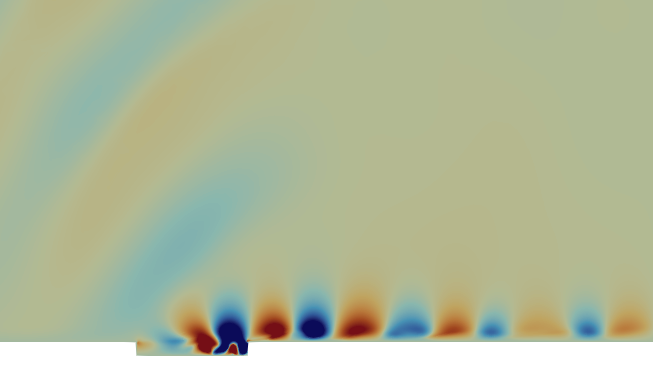
\includegraphics[width=\linewidth]{Images/d2.5_w20_Ma0.6.png}
		\end{column}
		\begin{column}{0.49\linewidth} % Left column
		  $w = 20$, Ma = 0.8:
		  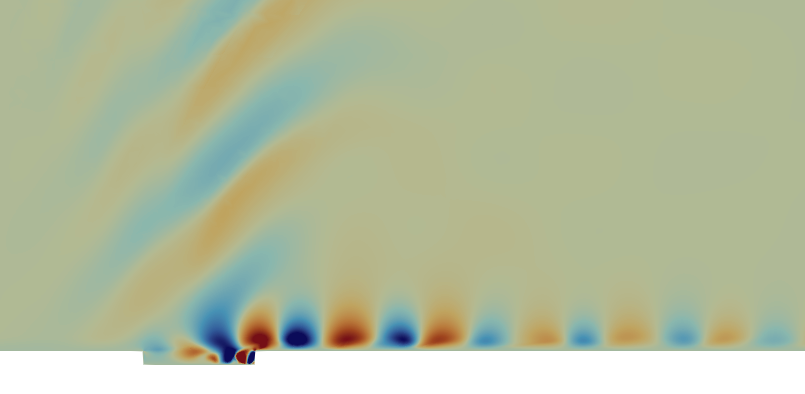
\includegraphics[width=\linewidth]{Images/d2.5_w20_Ma0.8.png}
		  $w = 29$, incompressible:
		  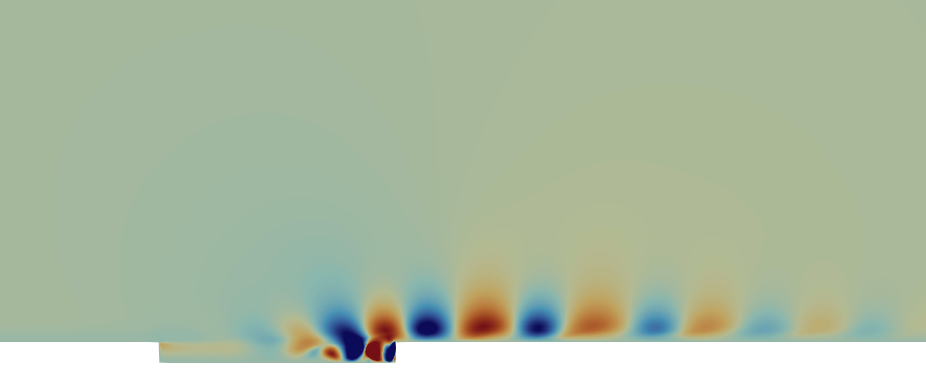
\includegraphics[width=\linewidth]{Images/d2.5_w29_inc.png}
		\end{column}  
	\end{columns}

\end{frame}
\begin{frame}
  \frametitle{Unstable mode 3d $d=3$, $w=10$}
  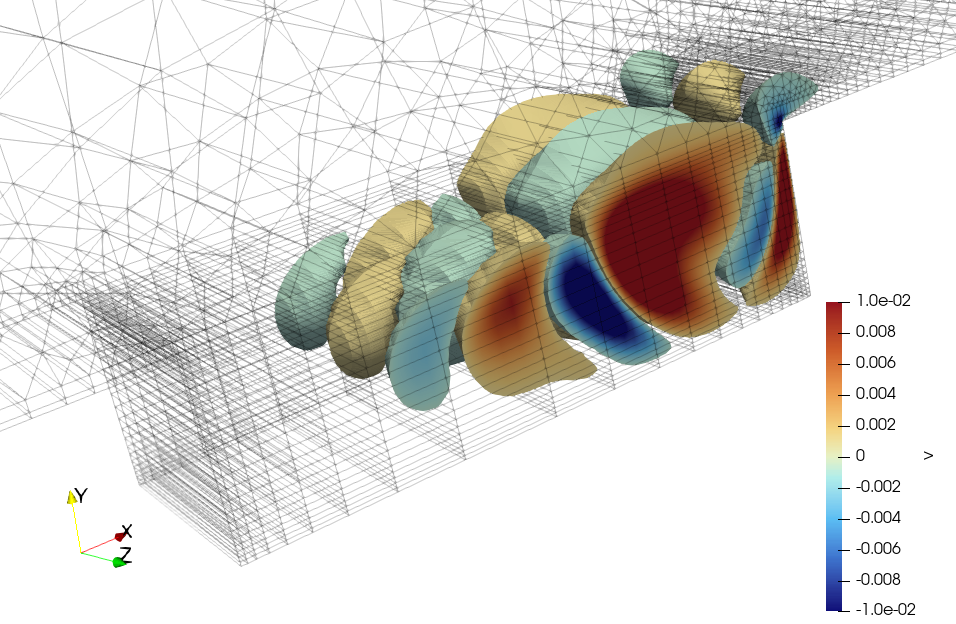
\includegraphics[width=0.8\linewidth]{Images/d3_w10_3d.png}
\end{frame}
\end{document}
